\documentclass[11pt, conference]{IEEEtran}
\usepackage{xeCJK}
\usepackage{amsmath}
\usepackage{listings}
\usepackage{amssymb}
\usepackage{float} %用来让图片显示在指定文字下面


% 用来断词,当出现花括号中的单词时,若遇到换行需要断词的话就只能从-处断。
\hyphenation{op-tical net-works semi-conduc-tor}

\begin{document}
    \title{Report 4: Invariant}
    \author{\IEEEauthorblockN{林奇峰, Qifeng Lin}\IEEEauthorblockA{Student ID:17214656}}
    \date{\today}
    \maketitle

    \section{Review}
        According to the entry of "invariant" in Wikipedia, the definition is that, {\itshape In computer science, an invariant is a condition that can be relied upon to be true during execution of a program, or during some portion of it. }

        To explain intuitively, an example of MU puzzle is introduced. MU puzzle is defined as following:

        Suppose there are the symbols M, I, and U which can be combined to produce strings of symbols. The MU puzzle asks one to start with the "axiomatic" string {\textbf MI} and transform it into the string {\textbf MU} using in each step one of the following transformation rules:
        \begin{figure}[H]
            \centering
            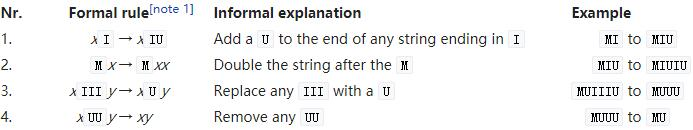
\includegraphics[width=3.5in]{1.jpg}
        \end{figure}

        Manually computing the possibility is available but we want to find a property that is invariant for all transformation rules. By observing if the transformation rule satisfies the property,we can reason the answer of the problem. It can be observed that if the number of I's in the string is always not a multiple of 3, then getting to {\textbf MU} is impossible. Therefore, define an invariant that during execution, {\itshape the number of I's in the string is not a multiple of 3.} If the program always holds the invariant, then it cannot be transformed into {\textbf MU}. Then, a table of the four rules is listed.
        \begin{figure}[H]
            \centering
            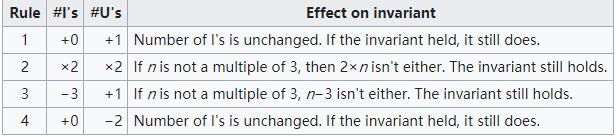
\includegraphics[width=3.5in]{2.jpg}
        \end{figure}

        For rule 1, it is obvious that rule 1 still holds the invariant if it has owned. As for rule 2, the invariant is still be held because 2 is not the multiple of 3. And rule 3 decreases "I" by 3 and the number of "I" is still not a multiple of 3. Rule 4 is the same as rule 1. Then, we can conclude that for the four transformation rules, if the invariant exits during executions, then getting to {\textbf MU} is impossible.

        The program written in C can be showed as following picture:
        \begin{figure}[H]
            \centering
            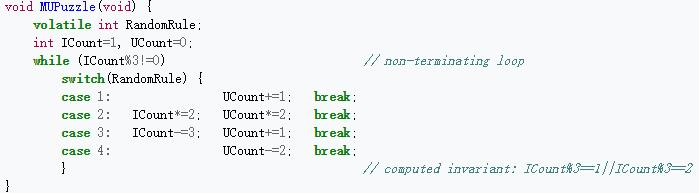
\includegraphics[width=3.5in]{3.jpg}
        \end{figure}

        If the loop cannot be terminated, it means that the program holds the invariant and thus cannot transform {\textbf MI} into {\textbf MU}.

        Therefore, we can define some invariants we want the program holding to ensure the result we want.

    \section{Summary}
        Invariant is a property that should be held during a phase of execution. And we can reason about the correctness of program by using the invariant. And in $\text{CTL}^*$, invariant can be expressed as \textbf{AG}. If we can find a path violating the property, then the invariant is false.

\end{document} 